
\documentclass[12pt]{article}
\usepackage{fullpage,amsmath,amssymb,graphicx}

\usepackage{setspace}
\spacing{1}

\usepackage{textpos}
\usepackage{tikz}
\usepackage{pgf}
\usepackage{amssymb}
\usepackage{enumerate}
\usepackage{xcolor}
\usepackage{graphicx}
\usepackage{subcaption}
\usepackage{tabularx}
\usepackage{colortbl}
\usepackage{multicol}
\usepackage{longtable}
\usepackage{hyperref}
\usepackage{comment}
\usepackage{listings}



\definecolor{encabezado}{rgb}{0.74, 0.83, 0.9}

\begin{document}

\hfill\\
\rule{\textwidth}{1.5pt}

\begin{minipage}[t]{85mm}
  \begin{tabular}{l}
    \textbf{\large Instituto Tecnológico de Costa Rica} \\  
    \textbf{Escuela de Ingeniería Electrónica} \\
    \textbf{Trabajo Final de Graduación} \\
    \textbf{Proyecto:} Método basado en aprendizaje reforzado \\para el control automático de una planta no lineal. \\
    \textbf{Estudiante:} Oscar Andrés Rojas Fonseca \hspace{3cm}\rule{4.5cm}{1.5pt}\\
    I Semestre 2024 \hspace{8.5cm}\textbf{Firma del asesor}
  \end{tabular}
\end{minipage}
\hfill\\
\rule{\textwidth}{1.5pt}


\section*{Bitácora de trabajo}

%\begin{table}[h]
\begin{minipage}[h]{\textwidth}
	\centering
	\begin{tabularx}{\textwidth}{|p{2cm}|X|X|p{2cm}|} 
		\hline
		\rowcolor{encabezado}
		\textbf{Fecha} & 
		\textbf{Actividad} & 
		\textbf{Anotaciones} & 
		\textbf{Horas dedicadas} \\ \hline
		% ***************************************************************
	 	15/04/2024 & 
	 	$\mathbf{1}.$ Redefinición de la conversión del código para valores discretos ($CartPole$) a valores continuos ($Pendulum$). & 
	 	$a)$ El error en $select\_ action()$ se corrigió pero desconfiguró parte de la función $optimize\_ model()$. Corrección del error. \newline
	 	$b)$ Persisten los problemas de indexado y proceso. \newline & 
	 	6 horas \\
	 	% ***************************************************************
	 	15/04/2024 & 
	 	$\mathbf{2}.$ Pruebas de entrenamiento del modelo ($Pendulum$). & 
	 	$a)$ Se entrenaron cuatro modelos diferentes a $600$ episodios para comparar el efecto de cuatro propuestas de redes neuronales artificiales (ANN). \newline & 
	 	4 horas \\
		% ***************************************************************
		16/04/2024 & 
	 	$\mathbf{3}.$ Búsqueda de la teoría de los métodos $PPO$ y $actor-critic$ dada la necesidad del manejo del \textit{action space} con valores continuos. &
	 	$a)$ Revisión general de los conceptos para ambos casos. Fuente importante en publicación de \href{https://medium.com/analytics-vidhya/coding-ppo-from-scratch-with-pytorch-part-1-4-613dfc1b14c8}{$PPO$} \cite{PPObeginners}. \newline
	 	$a)$ La fuente \cite{PPObeginners} facilita un enlace al repositorio de GitHub respectivo con ejemplos debidamente documentados. \newline & 
	 	4 horas \\
	 	% ***************************************************************
	 	17/04/2024 & 
	 	$\mathbf{4}.$ Reunión de seguimiento con el asesor del proyecto. & 
	 	$a)$ Revisión de avance en el código y errores de forma.  \newline
	 	$b)$ Se acordó continuar con el interés en los métodos como $PPO$ como opción. & 
	 	2 horas \\
		% ***************************************************************

	 	\hline
	\end{tabularx}
\end{minipage}	 	
	 	
	 	% ***************************************************************
\hfill\\
\begin{minipage}[h]{\textwidth}
	\centering
	\begin{tabularx}{\textwidth}{|p{2cm}|X|X|p{2cm}|} 
		\hline		
		
	 	% ***************************************************************
	 	17/04/2024 & 
	 	$\mathbf{5}.$ Búsqueda de métodos para el manejo de valores continuos en $DQN$. &
	 	$a)$ Las opciones popularmente mencionadas son el \textit{actor-critic} y el $DDPG$. Se procede a investigar $DDPG$ \newline
	 	$b)$ La opción de discretizar el \textit{action space} también se menciona. \newline & 
	 	4 horas \\
	 	% ***************************************************************
	 	17/04/2024 & 
	 	$\mathbf{6}.$ Prueba de discretización del \textit{action space} del env $Pendulum$. &
	 	$a)$ Se logró adaptar el código del $PendulumDQN$ a una versión discretizada $PendulumDQN\_discrete$, depende principalmente de la resolución seleccionada ($n\_actions$). \newline
	 	$b)$ Pruebas de entrenamiento de hasta $100$ episodios. \newline & 
	 	6 horas \\
	 	% ***************************************************************
	 	19/04/2024 & 
	 	$\mathbf{7}.$ Revisión de implementación del $DDPG$ y el $PPO$. &
	 	$a)$ Se buscaron ejemplos para aplicar \href{https://pytorch.org/tutorials/advanced/coding_ddpg.html?highlight=ddpg}{$DDPG$} mediante PyTorch para evitar ajustes innecesarios. \newline
	 	$b)$ Estudio de otros repositorios para aplicar \href{https://github.com/vwxyzjn/ppo-implementation-details/tree/main}{$PPO$}. \newline & 
	 	4 horas \\
	 	% ***************************************************************
	 	20/04/2024 & 
	 	$\mathbf{8}.$ Montaje y primera prueba del código \href{https://github.com/ericyangyu/PPO-for-Beginners/tree/master}{$PPO$} para $Pendulum$. &
	 	$a)$ Revisión del error por cambio de versión $Gym$ a $Gymnasium$. \newline
	 	$b)$ Implementación del procesamiento $CUDA$ en el código. \newline & 
	 	8 horas \\
	 	% ***************************************************************
	 	21/04/2024 & 
	 	$\mathbf{9}.$ Prueba de entrenamiento con versión base del $PPO$ para $Pendulum$. &
	 	$a)$ Entrenamiento del modelo con $render("human")$ de $200k$ episodios. Mal desempeño. \newline
	 	$b)$ Entrenamiento del modelo con $render("rgb\_ array")$ de $200M$ de episodios. Interrumpido por tiempo. \newline & 
	 	6 horas \\
	 	% ***************************************************************   
	 	\hline       
	\end{tabularx}
\end{minipage}
%\end{table}



\hfill\\
\begin{minipage}[h]{\textwidth}
	\centering
	\begin{tabularx}{\textwidth}{|p{2cm}|X|X|p{2cm}|} 
		\hline		
	 	% ***************************************************************
	 	21/04/2024 & 
	 	$\mathbf{10}.$ Adición de la función $calculate\_reward()$ al código base $PPO$ de $Pendulum$. &
	 	$a)$ Ajuste de la función para retornar valores $float$, no $torch.tensor()$. \newline
	 	$b)$ Ajuste de las funciones $log\_summary()$ para una mejor apreciación del proceso de entrenamiento y prueba. \newline
	 	$c)$ Estudio del uso de $Tensorboard$ para procesos de entrenamiento de \textit{Machine Learning}. \newline & 
	 	6 horas \\
	 	% ***************************************************************
	 	22/04/2024 & 
	 	$\mathbf{11}.$ Pruebas de implementación del método \href{https://github.com/schneimo/ddpg-pytorch/tree/master}{$DDPG$} para $Pendulum$. &
	 	$a)$ Montaje del código en carpeta $PruebasDDPG$ y se realizaron las primeras pruebas de entrenamiento. Errores de forma en el proceso. \newline & 
	 	4 horas \\
	 	% ***************************************************************
	 	22/04/2024 & 
	 	$\mathbf{12}.$ Pruebas de entrenamiento de $PendulumPPO$. &
	 	$a)$ Entrenamiento de modelo con $1M$ de episodios. Se muestra con avance prometedor en cuanto a las $rewards$. \newline & 
	 	6 horas \\
	 	% ***************************************************************
	 	23/04/2024 & 
	 	$\mathbf{13}.$ Pruebas montaje e incorporación del código $pahm\_model.py$ proporcionado por el profesor asesor. &
	 	$a)$ Primeras pruebas de implementación y adición del proceso método $PPO$ al entrenamiento. \newline & 
	 	4 horas \\
	 	% ***************************************************************
	 	
	 	\hline
		\multicolumn{3}{|r|}{Total de horas de trabajo:} & 64 horas \\ 
	 	\hline                 
	\end{tabularx}
\end{minipage}





% *****************************************************************************
% *****************************************************************************
% *****************************************************************************

\section*{Contenidos de actividades}

\subsection*{Primera prueba de entrenamiento $PPO$}

El código base utilizado \cite{PPObeginners} cuentaba con un valor de \textit{timesteps} por defecto de docientos millones ($200M$), por lo que luego de adaptar el código para su funcionamiento mediante el procesamiento $CUDA$, se probó cumplir con esta cantidad, como se observa en la Figura \ref{fig:PendPPOv1}.

\begin{figure}[h!]
	\centering
	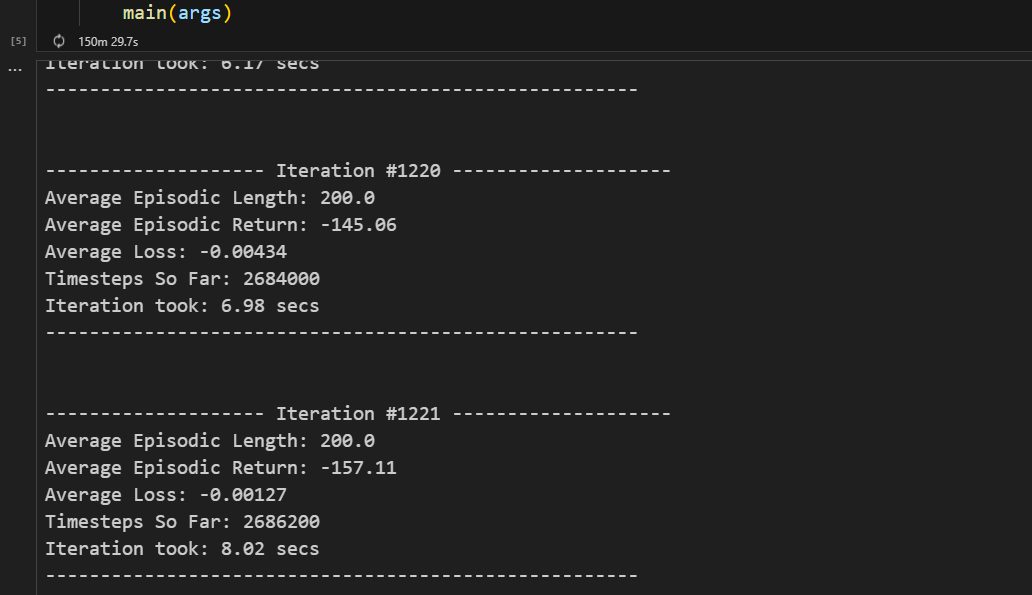
\includegraphics[scale=0.45]{Fig/Captura_PPO_200Me.png}
	\caption{Proceso de entrenamiento del modelo para $PendulumPPO$ con $200M$ de episodios.}
	\label{fig:PendPPOv1}
\end{figure}	

Sin embargo y apesar de observarse un avance en el entrenamiento, luego de un aproximado de tiempo de cuatro horas transcurridas se proyectó un faltante importante, por lo que se decidió interrumpir el proceso para lograr mejoras en otros puntos del proyecto.

\subsection*{Ajuste en la función $log\_summary()$ de $PPO$}

Se buscó una mejora en la forma de monitoreo del avance del entrenamiento del modelo, por lo que agregó la lógica de la librería $Matplotlib$ y se probó con un entrenamiento inicial de $100k$ episodios como se muestra en la Figura \ref{fig:PendPPOv2}.

\begin{figure}[h!]
	\centering
	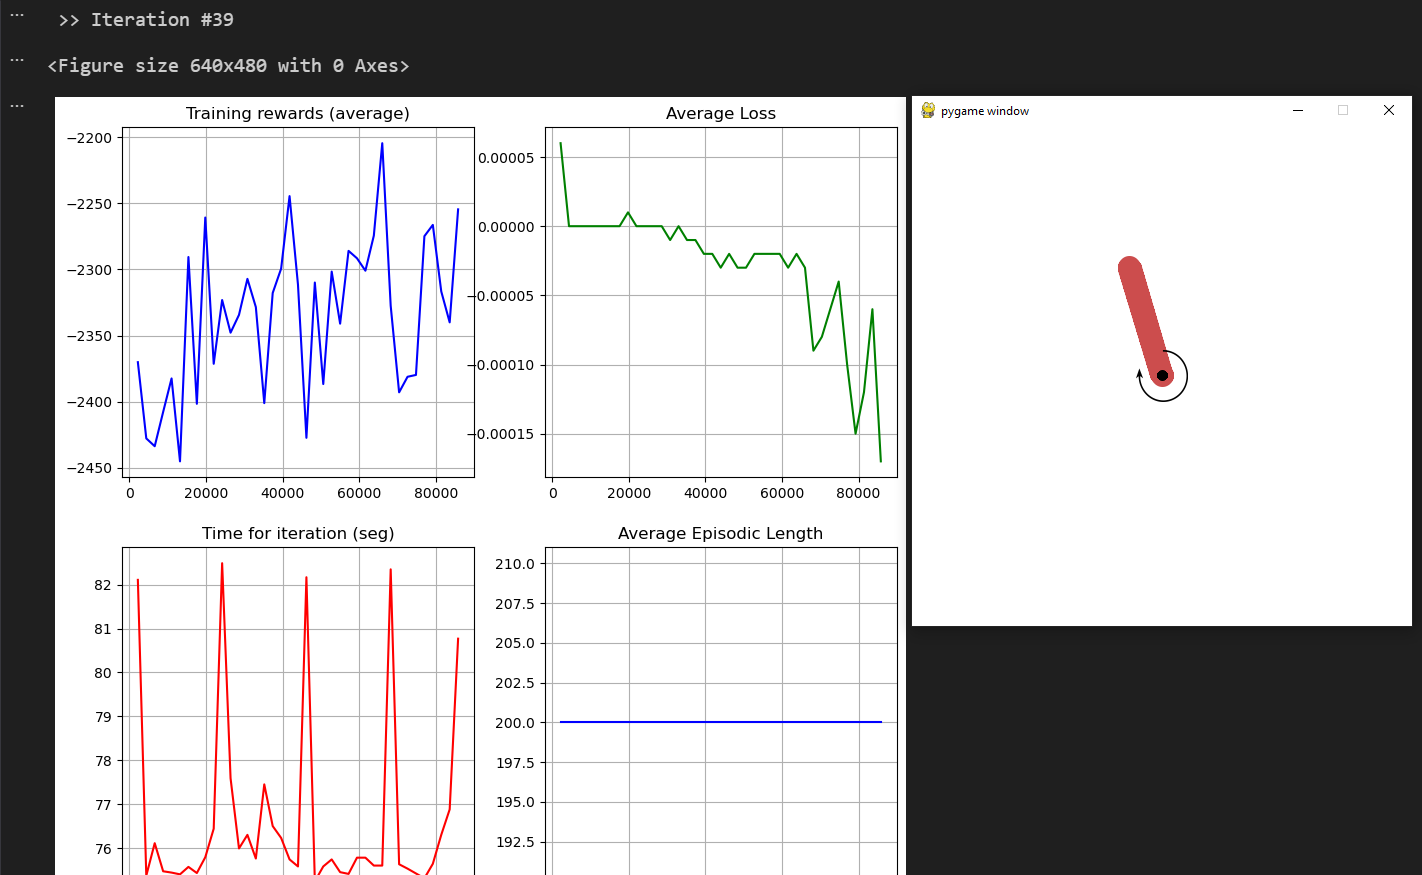
\includegraphics[scale=0.35]{Fig/Captura_PPO_100ke_updated.png}
	\caption{Proceso de entrenamiento del modelo para $PendulumPPO$ con $100k$ episodios.}
	\label{fig:PendPPOv2}
\end{figure}

También se empezó con pruebas simples de monitoreo mediante la librería $Tensorboard$, las cuales se encuentran en proceso.

\subsection*{Entrenamiento de modelo $PPO$ de $1M$ de episodios}

Luego de ajustar el monitoreo y agregar la lógica del $target\_angle$ al código, se procedió a entrenar un modelo con $1$ millon de episodios y fijar el ángulo en $135^o$,  Figura \ref{fig:PendPPOv3}, mostrando un desempeño prometedor.

\begin{figure}[h!]
	\centering
	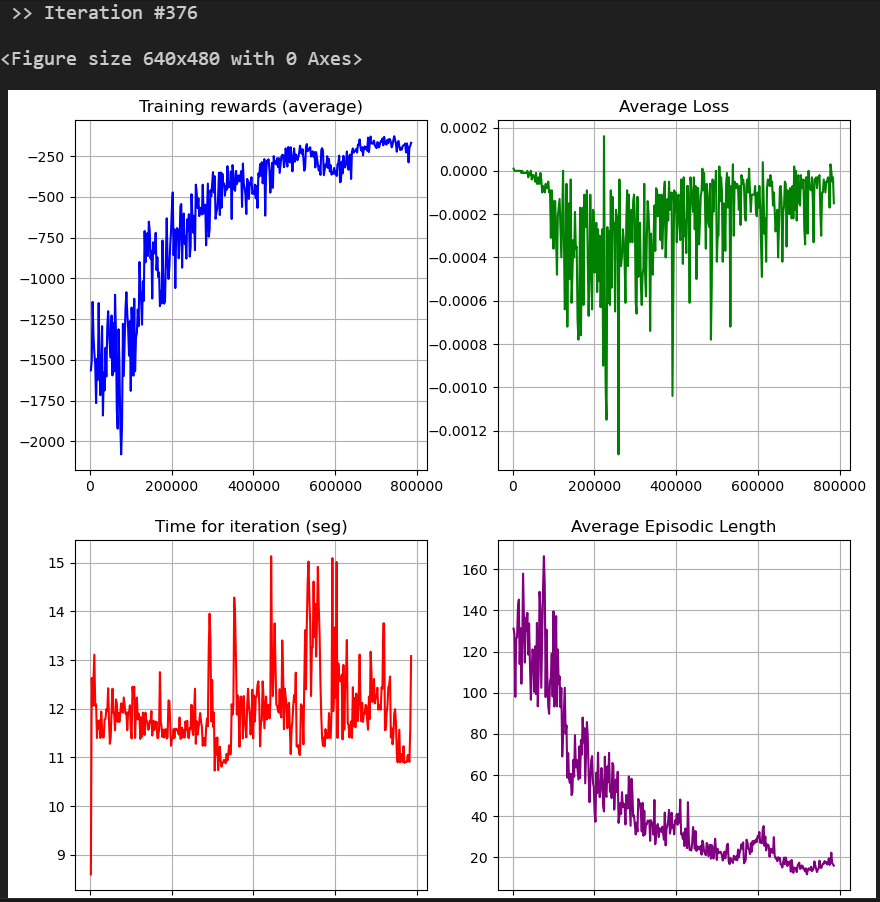
\includegraphics[scale=0.45]{Fig/Captura_PPO_1Me_135d.png}
	\caption{Proceso de entrenamiento del modelo para $PendulumPPO$ con $1M$ de episodios y $target\_angle=135$.}
	\label{fig:PendPPOv3}
\end{figure}	

Se encuentra en proceso de implementación la variación constante del ángulo y más entrenamientos, dada la necesidad de periodos largos de tiempo para entrenamientos de modelos prometedores.

\newpage

\section*{Referencias}
\renewcommand\refname{}
\bibliographystyle{IEEEtran}
\bibliography{references}





\end{document}
